%% Philipp G Freimann Juli 2019 für die BBW
%% Phi BBW-Vorlage für Arbeitsblätter (LaTeX)
%% 2019 - 08 - 18

%% %% %% %%


%%  In den Dokumenten können die folgenden Attribute überschrieben werden:


\newcommand{\metaHeaderLine}{HeaderLine mit $\backslash{}$ metaHeaderLine überschreiben}

%% \thema
\newcommand{\arbeitsblattTitel}{Pruefungsthema mit renewcommand
  arbeitsblattTitel überschreiben.}


%%%%%%%%%%%%%%%%%%%%%%% P A C K A G E S %%%%%%%%%%%%%%%%%%%%%%%%%%%%%
\usepackage[paper=a4paper,margin=17mm]{geometry}

%%\usepackage{german} %% Macht Probleme mit grafiken
\usepackage{mciteplus}

\usepackage[dvipsnames]{xcolor}

\usepackage{pgfplotstable}
\usepackage{tikz}
\usepackage{tkz-euclide} %% Grid

\usepackage{amsthm}
\usepackage{amsfonts} %% Zahlmengen Z, R, ...


%% THEOREMS?
\usepackage{tcolorbox}
\tcbuselibrary{theorems}
\tcbuselibrary{skins}


\usepackage{fancyhdr}
\usepackage{ngerman}
\usepackage[utf8]{inputenc}


%%\usepackage[dvips]{graphicx}

\usepackage{supertabular}
\usepackage{makeidx}  
\usepackage{ifthen} 

\usepackage{multirow}
\usepackage{listings}

%%\usepackage{color,fancyvrb,fancybox}
\usepackage{multicol}
\usepackage{lastpage}
%%\usepackage{listings}
\usepackage{pstricks}

%% bold typewriter font:
\usepackage[T1]{fontenc}
\usepackage{lmodern}

\usepackage{enumitem}
%\usepackage{enumerate}

\usepackage{float}

\usepackage{titlesec}
\usepackage{textcomp}

%% Kuchendiagramme
%%\usepackage{datapie}

%% für Aufgaben Hervorhebung
%%\usepackage[most]{tcolorbox}
%%\usepackage[standard,framed]{ntheorem}
\usepackage{framed}
\usepackage{mdframed}

%%%%%%%%%%%%%%%%%%%%
%%\usepackage[most]{tcolorbox}

\usepackage[tocindentauto]{tocstyle}

%% für accentset wedge:
\usepackage{accents}

%% Würfel
\usepackage{epsdice}

%% Einbinden von GeoGebra Bildchen:
\usetikzlibrary{shapes.geometric}
\usetikzlibrary{arrows}
\newcommand{\degre}{\ensuremath{^\circ}}

%% Hyperlinks
\usepackage{hyperref}

\hypersetup{
    colorlinks=true,
    linkcolor=blue,
    filecolor=magenta,      
    urlcolor=cyan,
    bookmarks=true,
}

%% bugtracker (part of pgfplots) should be loaded AFTER "hyperref"
%% See: https://texblog.net/hyperref/ AND https://tex.stackexchange.com/questions/16268/warning-with-footnotes-namehfootnote-xx-has-been-referenced-but-does-not-exi
\usepackage{pgfplots}
\pgfplotsset{width=10cm,compat=1.9}


\usepackage{tgheros}%% Font TeX Gyre Heros für Titel (font code qhv)

%% damit die Punktezal schon geschrieben werden kann, obschon
%% Die Punkte erst während dem Dokument zusammengetragen werden:

%%%%%%%%%%%%%%% L A Y O U T  %%%%%%%%%%%%%%%%%%%%%%%%%%%%
%% 2020-12-27 ph. g. freimann @ bbw.ch
%%

\fancyhf{}%%

\pagestyle{fancy}%%

\renewcommand{\sectionmark}[1]{%%
  \markboth{\thesection{} \ #1}{}%%
}%%

\renewcommand{\subsectionmark}[1]{%%
  \markright{\thesubsection \ #1}%%
}%%

%% Achtung: chaptermark nur im BOOK-Style

\renewcommand{\footrulewidth}{0.4pt}

\parskip4pt
\parindent0pt

\topmargin-2.0cm
\textheight24.4cm

\renewcommand{\arraystretch}{1}%%

%%%%%%%%%%%%%%%%%%%%%%%%%%%%%%%%%%%%%%%%%%%%%%%%%%%%%%%%%%
%%%%%%%%%%%%%%%%%% M A K R O S %%%%%%%%%%%%%%%%%%%%%%%%%%%
%%%%%%%%%%%%%%%%%%%%%%%%%%%%%%%%%%%%%%%%%%%%%%%%%%%%%%%%%%

%%%%%%%%%%%%%%%%%%%%%%%% g e n e r e l l e   M a k r o s %%%%%%%%%%%%%%%%%%%%%%%

%% 2019-07-26
%% phi@freimann.eu
%% Makros for BBW-Tex Documents
\usepackage{inputs/bbwColors}

%%%%%%%%%%%%%%%%%% I N C L U D E S   &   I N D E X  %%%%%
\graphicspath{{../img/}}
\graphicspath{{./img/}}

\newcommand\bbwGraphicRaise[3]{\raisebox{#1}{\includegraphics[width=#2]{#3}}}%%
\newcommand\bbwGraphic[2]{\bbwGraphicRaise{-5mm}{#1}{#2}}%%
\newcommand\bbwCenterGraphicRaise[3]{\begin{center}\bbwGraphicRaise{#1}{#2}{#3}\end{center}}
\newcommand\bbwCenterGraphic[2]{\bbwCenterGraphicRaise{-5mm}{#1}{#2}}%%


%% All in one Skript
\newif\ifisALLINONE
\isALLINONEfalse

%%%%%%%%% TRAINER Version vs. Schülerversion %%%%%%%%%%%%%

\newcommand\TRAINER[1]{%%
{%%
\ifisTRAINER{\color{BlueGreen}{#1}}%%
\fi%%
}}%%  

\newcommand\TALS[1]{%
{%%
\ifisTALS {#1}%%
\fi%%
}}%

\newcommand\GESO[1]{%
{%%
\ifisGESO {#1}%%
\fi%%
}}%    

\newcommand{\noTRAINER}[1]{{\ifisTRAINER{}\else{#1}\fi}{}}%%



%%\makeatletter
%% Je nach Umgebung "environment" wird das mmPapier breiter oder
%% schmaler
%% bei itemize sollen 16.4 und bei definiton-Boxen 16.8 mm genommen
%% werden.


\usepackage{inputs/mmPapierbreiteSty}


%% Trainer "no" Dotfill
%% If no Trainer: Dotfill
\newcommand{\TNDF}[1]{\TRAINER{#1}\noTRAINER{\dotfill{}}}%%

\newcommand{\leserluft}{\vspace{2mm}}

%% Notiz felder 
%% Anwendung:
%% \noteField{10}  
%%  --> Notizfeld mit 10 Leerzeilen
\newcounter{DFCounter}

\newcommand*{\noteField}[1]{%
\setcounter{DFCounter}{1}
\vspace{0.5in}%
\begin{tabular}{p{14cm}}%
\hline%
\vspace{0.2cm}
Notizen: \\%
\whiledo{\theDFCounter < #1}{%
\dotfill \\
\addtocounter{DFCounter}{1}%
}%
\end{tabular}%
}%

\newcommand*{\noteLines}[1]{%
\setcounter{DFCounter}{1}
\vspace{0.1cm}%
\begin{tabular}{p{14cm}}%
\whiledo{\theDFCounter < #1}{%
\dotfill \\
\addtocounter{DFCounter}{1}%
}%
\end{tabular}%
}%

%% Platz für Notizen, aber nur bei Schülernverison (\noTRAINER)
\newcommand{\platzFuerTNNotes}[1]{%
\ifisTRAINER{}\else{%%
Platz für Notizen:\newline%%
\noteLines{#1}%%
}\fi{}%
}%%

%% Vier Leerzeilen für Notizen
\newcommand*\dotfillpara{%
\begin{tabular}{p{11.5cm}}%
\hfill   \\
\dotfill \\
\dotfill \\
\dotfill \\
\dotfill
\end{tabular}%
}


%%Häuschenpapier
\newcommand{\mmPapierZwei}[2]{\begin{tikzpicture}
%%  \draw[step=4mm,bbwMMFarbe,ultra thin]
%%  \draw[step=4mm,bbwMMFarbe,thick]
  \draw[step=4mm,bbwMMFarbe,line width=0.02mm]
  (0, 0) grid ({#2}, {#1});
\end{tikzpicture}}%%


%% millimeterPapier füllen bis Ende Seite
\newcommand{\mmPapierBisEndeSeite}{

\begin{tikzpicture}

\newdimen\spaceleftOnPage
\spaceleftOnPage=\dimexpr\textheight-\pagetotal-14pt\relax

\pgfmathsetmacro{\gridWidth}{\textwidth        - mod(\textwidth,      4mm)      }
\pgfmathsetmacro{\gridHeight}{\spaceleftOnPage - mod(\spaceleftOnPage,4mm) - 4mm}

\draw [step=4mm,bbwMMFarbe,line width=0.02mm] (0,0) grid (\gridWidth pt,\gridHeight pt);
\end{tikzpicture}%%
\newpage%%
}%% END Makro mmPapieBisEndeSeite


%% Standardbreite für Arbeitsblätter und das Theorieheft
%% Wird in bbwPruefung.sty überschrieben, da dort schmaler
\def\defaultTextBreite{17.6}
\def\unitCMWhatElse{cm}%% wird als Breitenangabe für den nächsten command verwendet

%% Verwendung: \bbwCenterGraphic{\defaultTextBreite}{«img url»}
\def\defaultTextBreiteCM{\defaultTextBreite\unitCMWhatElse}
\newcommand{\mmPapier}[1]{\mmPapierZwei{#1}{\defaultTextBreite}}


%% Notizen Berechungen auf Prüfungsblättern
\newcommand{\platzFuerBerechnungen}[1]{\noTRAINER{

Notizen / Berechnungen:

\mmPapier{#1}}}%% end platzFuerBerechnungen

\newcommand{\platzFuerBerechnungenBisEndeSeite}[1]{\noTRAINER{

Notizen / Berechnungen:

\mmPapierBisEndeSeite}}%% end platzFuerBerechnungen



\newcommand{\platzFuerBerechnungenOhneText}[1]{\noTRAINER{

\mmPapier{#1}}}


%% Die Abkürzung z.\,B. von «Zum Beispiel» hat einen verkleinerten Abstand.
\newcommand*\zB{%
z.\,B.
}

%%
%% Auf der Titelseite steht entweder GESO oder TALS.
%% Dies wird gleich mit der Fußnote angegeben.
%% Dieses Kommando sollte im Kommando «\untertitel» eingesetzt werden.
%%
\newcommand*\ausrichtungAufTitelseite{%
\ifisTALS{TALS\noTRAINER{\footnote{TALS «Technik, Architektur und Life Sciences
(Laboranten)»: Ausrichtung technisches Profil}}}%%
\fi%%
\ifisGESO{GESO\noTRAINER{\footnote{GESO: Ausrichtung \textbf{Ge}sundheit und \textbf{So}ziales}}}%%
\fi}%%

%%%%%%%%%%%%%%%%%%%%%% B B W - M a t h e   F a r b c o d e s  %%%%%%%%%%%%%%%%%%%%%%%%%%%%%%555

\newcommand{\rezeptFarbe}{rezeptFarbe}
\newcommand{\definitionFarbe}{definitionFarbe}
\newcommand{\gesetzFarbe}{gesetzFarbe}
\newcommand{\beispielFarbe}{beispielFarbe}
\newcommand{\bemerkungFarbe}{bemerkungFarbe}

%% Falls gewünscht übersteuren
%  \definecolor{xyz}{HTML}{eeff66}
%  \renewcommand{\beispielFarbe}{xyz}
%

%% Theorem-Styles
\newcommand\theoremlayoutdefinition[4]{\newtcbtheorem[number within=section]{#1}{#2}%
   {theorem style=plain,enhanced,colframe=#3!20!white,colback=#3!20!white,
     coltitle=#3!60!black,fonttitle=\upshape\bfseries,
     %%fontupper=\itshape,
    %%drop fuzzy shadow=blue!50!black!50!white,
    terminator sign={:},
    borderline north={0.5mm}{0pt}{#3}, borderline south={0.5mm}{0pt}{#3}
   }{#4}}



%% Farben für rezept, definition und gesetz von Marthale übernommen.
%% Verwendung mit * unterbindet die Nummerierung \begin{gesetz*}{Blah}{xy} ...\end {gesetz*}
\theoremlayoutdefinition{rezept}{Rezept}{\rezeptFarbe}{R}
\theoremlayoutdefinition{definition}{Definition}{\definitionFarbe}{D}
\theoremlayoutdefinition{gesetz}{Gesetz}{\gesetzFarbe}{G}%% was green
\theoremlayoutdefinition{beispiel}{Beispiel}{\beispielFarbe}{B}
\theoremlayoutdefinition{bemerkung}{Bemerkung}{\bemerkungFarbe}{M}


%% AadB = Aufgaben aus dem Buch
%% 1. Parameter: Seitenzahl
%% 2. Parameter: Aufgabennummern.
%% bsp  \TALSAadB{38-39}{101a-101c, 102 und 103}



%%\newcommand*{\maturaAufgaben}[1]{\begin{mdframed}[backgroundcolor=maturaAufgabenFarbe!10]{#1}\end{mdframed}}

\newcommand*{\aadB}{Aufgaben aus dem Buch}

\newcommand*{\TALSAadB}[2]{%%
{%%
\ifisTALS{\aufgabenFarbe{\noindent{\aadB \cite{frommenwiler17alg}: Seite {#1} Nr. {#2}}}}%%
\fi%%
}}%%

\newcommand*{\TALSGeomAadB}[2]{%%
{%%
\ifisTALS{\aufgabenFarbe{\noindent{\aadB \cite{frommenwiler18geom}: Seite {#1} Nr. {#2}}}}%%
\fi%%
}}%%

\newcommand*{\GESOAadB}[2]{%%
{%%
\ifisGESO{\aufgabenFarbe{\aadB \cite{marthaler21}: Seite {#1} Nr. {#2}}}%%
\fi%%
}}%%

\newcommand*{\theorieGESO}[2]{%%
{\ifisGESO{Theorie \cite{marthaler21}: Seite {#1} Kap. {#2}}%%
\fi%%
}}

\newcommand*{\theorieTALS}[2]{%%
{\ifisTALS{Theorie \cite{frommenwiler17alg}: Seite {#1} Kap. {#2}}%%
\fi%%
}}

\newcommand*{\theorieTALSGeom}[2]{%%
{\ifisTALS{Theorie \cite{frommenwiler18geom}: Seite {#1} Kap. {#2}}%%
\fi%%
}}

%%
%% Force a blank page, when \newpage does not work
%%
\def\blankpage{%
	\clearpage%
	\null%
	\clearpage}%%

\newcommand{\Lueckentext}[1]{\,\,\noTRAINER{\dotfill}\TRAINER{#1}}

\newcommand{\LoesungsRaum}[1]{\,\,\noTRAINER{\underline{\underline{\,\,\,\,\,\,\,\,\,\,\,\,\,\,\,\,\,\,\,\,\,\,\,\,\,\,}}}\TRAINER{#1}\,\,}

\newcommand{\LoesungsRaumKurz}[1]{\,\,\noTRAINER{\underline{\underline{\,\,\,\,\,\,\,\,\,\,\,}}}\TRAINER{#1}\,\,}

\newcommand{\LoesungsRaumLang}[1]{\,\,\noTRAINER{\underline{\underline{\,\,\,\,\,\,\,\,\,\,\,\,\,\,\,\,\,\,\,\,\,\,\,\,\,\,\,\,\,\,\,\,\,\,\,\,\,\,\,\,\,\,\,\,\,\,\,\,\,\,}}}\TRAINER{#1}\,\,}


%% TI nSpire
\def\tinspire{\texttt{TI-nSpire}}

%% TI 30 Pro Mathprint Button Images
\def\tiprobuttonbreite{10mm}
\def\nspirebuttonbreite{8.6mm}

%%\def\sec{\raisebox{-2mm}{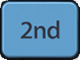
\includegraphics[width=\buttonbreite{}]{img/tiprobuttonimages/2nd.png}}}
\newcommand{\tiprobutton}[1]{\raisebox{-2mm}{\mbox{\,\includegraphics[width=\tiprobuttonbreite{}]{img/tiprobuttonimages/#1.png}\,}}}

\newcommand{\nspirebutton}[1]{\raisebox{-2mm}{\mbox{\,\includegraphics[width=\nspirebuttonbreite{}]{img/nspirebuttonimages/#1.png}\,}}}

%% Counter  für Aufgaben
%% Bei jedem Part wird die Aufgabennummer zurückgesetz auf 1
\newcommand{\bbwPartID}{AA1}
\newcommand{\bbwAufgabenBlockID}{}
\newcounter{bbwAufgabenNummerCounter}[part]
\setcounter{bbwAufgabenNummerCounter}{1}
\newcommand{\bbwAufgabenNummer}{\arabic{bbwAufgabenNummerCounter}}
\newcommand{\nextBbwAufgabenNummer}{\stepcounter{bbwAufgabenNummerCounter}}
\newcommand{\aufgSubLabel}{{\color{blue}\bbwAufgabenNummer. \alph*)}}

\newenvironment{bbwAufgabenBlock}{%% Begin environment

{\color{blue}\bbwAufgabenNummer. {\small[\bbwAufgabenBlockID]}}
\begin{enumerate}[label=\aufgSubLabel]
}{%% END Part
\end{enumerate}
\nextBbwAufgabenNummer
}%% END environment bbwAufgabenBlock

%%%%%%%%%%%%%%%%%%%%%%%%%%%%
%% Weblinks und Mathe Ninja Links

\newcommand{\weblink}[2]{\href{#2}{#1}}

\newcommand{\matheNinjaLink}[2]{
\begin{tabular}{cc}
 \raisebox{-1cm}{
\includegraphics[height=2cm]{img/matheninja/turtle.png}}& \href{#2}{MatheNinja: #1}\\
 \end{tabular} 
%%\bbwCenterGraphic{2cm}{img/matheninja/turtle.png}
%%$$\Longrightarrow \Longrightarrow \href{#1}{MatheNinja} \Longleftarrow\Longleftarrow$$
}%% End Command  \matheNinjaLink

%% Philipp G Freimann Juli 2019 für die BBW
%% Phi BBW-Vorlage für Mathematische Dokumente (LaTeX)
%% 2019 - 07 - 11
%%%%%%%%%%%%%%%%%%%%%%%%%%% M a t h e   M a k r o s %%%%%%%%%%%%%%%%%%%%%%%%%%%%%5

\usetikzlibrary{arrows.meta}

%% Kleine Symbole über anderen. Z. B. "?" über einem
%% Gleichheitszeichen:
%% Use \ueberMini{=}{?} um ein kleines Fragezeichen über ein
%% Gleichheitsszeichen zu schreiben.
\newcommand{\ueberMini}[2]{ \mathrel{\stackrel{\makebox[0pt]{\mbox{\normalfont\tiny #2}}}{#1}} }

%% Gleichungssystem mit zwei Zeilen und vier Einträgen (je zwei links
%% bzw. rechts).
\def\gleichungZZ#1#2#3#4{%%
  $$\left|
  \begin{array}{rcl}
    {#1} &=& {#2}\\
    {#3} &=& {#4}
    \end{array}\right|$$}%%

\def\gleichungDD#1#2#3#4#5#6{%%
  $$\left|
  \begin{array}{rcl}
    {#1} &=& {#2}\\
    {#3} &=& {#4}\\
    {#5} &=& {#6}\\
    \end{array}\right|$$}%%

%% Entspricht-Symbol
%%\usepackage{accents}
\newcommand{\hatset}[1]{\accentset{\wedge}{#1}}
\newcommand{\entspricht}{\,\,\hatset{=}\,\,}
\newcommand*\mittelwert[1]{\bar{#1}}
\newcommand*\mediantilde[1]{\widetilde{#1}}

%%
%% Graphiken mit tikz: BBW-Mathe-akros
%%
\tikzset{bbwgrid/.style={help lines,color=cyan!18, step=0.5cm}}

%% Koordinatensystem ohne Zahlen
\newcommand{\bbwGridPartLeer}[4]{
 % grid:
 \draw[bbwgrid] (#1,#3) grid (#2,#4);

 % axes
 \draw[thick] (#1,0) -- (#2,0);
 \draw[thick] (0,#3) -- (0,#4);
 \foreach \x in {#1, ..., -1}  \draw (\x cm, 2pt) -- (\x cm, -2pt);%%  node[anchor=north]{$\x$};
 \foreach \x in {1, ..., #2}   \draw (\x cm, 2pt) -- (\x cm, -2pt);%%  node[anchor=north]{$\x$};
 \foreach \y in {#3, ..., -1}  \draw (-2pt, \y cm) -- (2pt, \y cm);%%  node[anchor=east]{$\y\,\,$};
 \foreach \y in {1, ..., #4}   \draw (-2pt, \y cm) -- (2pt, \y cm);%%  node[anchor=east]{$\y\,\,$};
 \draw[->,thick] (#2,0) -- ({#2+0.5},0) node[anchor=west]{$x$};
 \draw[->,thick] (0,#4) -- (0,{#4+0.5}) node[anchor=south]{$y$};
}

\newcommand{\bbwGridPart}[4]{
 % grid:
 \draw[bbwgrid] (#1,#3) grid (#2,#4);

 % axes
 \draw[thick] (#1,0) -- (#2,0);
 \draw[thick] (0,#3) -- (0,#4);
 \foreach \x in {#1, ..., -1}  \draw (\x cm, 2pt) -- (\x cm, -2pt)  node[anchor=north]{$\x$};
 \foreach \x in {1, ..., #2}   \draw (\x cm, 2pt) -- (\x cm, -2pt)  node[anchor=north]{$\x$};
 \foreach \y in {#3, ..., -1}  \draw (-2pt, \y cm) -- (2pt, \y cm)  node[anchor=east]{$\y\,\,$};
 \foreach \y in {1, ..., #4}   \draw (-2pt, \y cm) -- (2pt, \y cm)  node[anchor=east]{$\y\,\,$};
 \draw[->,thick] (#2,0) -- ({#2+0.5},0) node[anchor=west]{$x$};
 \draw[->,thick] (0,#4) -- (0,{#4+0.5}) node[anchor=south]{$y$};
}


%% A function within a Grid (without painting the grid)
%% #1: funciton eg 2*\x  (x has to be backquoted)
%% #2: Domain eg. -1:2.5
%% #3: colour eg red
\newcommand{\bbwFuncC}[3]{\draw[domain=#2,smooth,samples=200,variable=\x,#3] plot ({\x},{#1});
}
%% A function within a Grid (without painting the grid)
\newcommand{\bbwFunc}[2]{\bbwFuncC{#1}{#2}{blue}}

%% Declare a function-plot
%% xmin,xmax,ymin,ymax,fct,domain(x-min, x-max)
%% example: \bbwFunction{-4}{3}{-2}{5}{-\x*\x- \x + 4.5}{-3:2}
\newcommand{\bbwFunction}[6]{\begin{tikzpicture}
\bbwGridPart{#1}{#2}{#3}{#4}
 \bbwFunc{#5}{#6}
%% \draw[domain=#6,smooth,samples=200,variable=\x,blue] plot ({\x},{#5});
\end{tikzpicture}}
%% a whole graph having a coordinate-system #1-#4 and any tizpicture content #5:
\newcommand{\bbwGraph}[5]{\begin{tikzpicture}\bbwGridPart{#1}{#2}{#3}{#4}#5\end{tikzpicture}}
\newcommand{\bbwGraphLeer}[5]{\begin{tikzpicture}\bbwGridPartLeer{#1}{#2}{#3}{#4}#5\end{tikzpicture}}

%% Dots and lines:
%% Dot example: \bbwDot{-1,2}{red}{east}{A}
\newcommand{\bbwDot}[4]{\filldraw[color=#2!60, fill=#2!5, thick](#1) circle(0.05) node[anchor=#3]{$#4$};}

%% Line example: \bbwLine{-1,0}{2,3}{red}
\newcommand{\bbwLine}[3]{\draw[thick,color=#3] (#1)--(#2);}

\newcommand{\bbwArrow}[3]{\draw[thick,color=#3,->] (#1)--(#2);}


%% Draw a single letter or small text
% #1: Position eg  4,4
% #2: letter eg f or blah
% #3: colour
\newcommand{\bbwLetter}[3]{\draw[color=#3](#1) node{$#2$};}

%%% ABC-Formel
%% usage \abcd{<a>}{<b>}{<c>}
%% example usage: \abcd{b}{5}{\sqrt{4}}
\newcommand{\abcd}[3]{$\frac{-(#2)\pm\sqrt{(#2)^2 - 4\cdot{}(#1)\cdot{}(#3)}}{2\cdot{}(#1)}$}



%% Trigonometrische Koordinatensysteme
%% Alle heißen "trigsysS" wobei da S einer der folgenden Sub-Systeme
%% bezeichnet:
%%  A  phi von  0 ... 360
%%     y   von -3 ...   3
%%
%%  B  phi von  0 ... 360
%%     y   von -1 ...   1
%%
%%  C  phi von  -270 ... 450
%%     y   von    -2 ...   2
%%
%%  D  phi von  -270 ... 450
%%     y   von    -1 ...   1
%%

%% coordSysBBWFlex
%% Flexibles Koordinatensystem mit Pfeilen und Pfeilbeschriftung, aber
%% noch ohne "ticks".
%% #1   : Rastergröße
%% #2-#5: Größe des Rasters in cm
%% #6   : Beschriftung in x-Richtung (in y-Richtung ist es immer y
%% #7   : Zu zeichnende Funktion
%% #8   : Ticks oder was sonst noch komplexeres in die Grafik muss
\newcommand{\bbwFunctionColour}{blue}
\newcommand{\coordSysBBWFlex}[8]{
\begin{tikzpicture}
\draw[step = #1,  thin, cyan!20] (#2, #4) grid (#3, #5);
\draw[thick, ->] (#2,0) -- (#3,0) node[anchor = west] {$#6$};
\draw[thick, ->] (0,#4) -- (0,#5) node[anchor = south] {$y$};
\draw[domain=#2:#3,smooth,samples=200,variable=\x,\bbwFunctionColour] plot ({\x},{#7});
#8;
\end{tikzpicture}
\renewcommand{\bbwFunctionColour}{blue}
}%% end coordSysBBW

%% Koordinatensystem von 0 - 360 Grad (y -Ricthung -1 bis 1
%% Die Funktion kann mit dem 1. Parameter eingegeben werden
\newcommand{\trigsysAFct}[1]{
\coordSysBBWFlex{0.5cm}{-1}{13}{-4}{4}{\varphi}{#1}{
  \foreach \x [evaluate=\x as \degree using int(\x*30)] in {1,...,12}{ 
    \draw (\x cm, 1pt) -- (\x cm, -1pt) node[anchor = north] {$\degree^\circ$};
  }
  \foreach \y in {-3,-2,-1,1,2,3}{
   \draw (1pt, \y cm) -- (-1pt, \y cm) node[anchor = east] {$\y$};
  }
}
}%% end trigsysC

%% Leeres Koordinatensystem (fct = 0)
\newcommand{\trigsysA}{\trigsysAFct{0}}


%% Koordinatensystem von -270 bis 450 Grad. In y-Richtung von -2 bis 2
%% Funktion wird mit #1-Parameter angegeben
\newcommand{\trigsysBFct}[1]{
\coordSysBBWFlex{0.5cm}{-1}{13}{-4}{4}{\varphi}{#1}{
  \foreach \x [evaluate=\x as \degree using int(\x*30)] in {1,...,12}{ 
    \draw (\x cm, 1pt) -- (\x cm, -1pt) node[anchor = north] {$\degree^\circ$};
  }
  \foreach \y in {-1,1}{
   \draw (1pt, \y *3cm) -- (-1pt, \y *3cm) node[anchor = east] {$\y$};
  }
}
}%% end trigsysC

%% Leeres B-System
\newcommand{\trigsysB}{\trigsysBFct{0}}


%% Wie B-SYstem, jedoch in y-Richtung von -1 bis +1
\newcommand{\trigsysCFct}[1]{
\coordSysBBWFlex{0.2cm}{-6}{10}{-2.5}{2.5}{\varphi}{#1}{
  \foreach \x [evaluate=\x as \degree using int(\x*90)] in {-3,-2,-1,1,2,3,4,5}{ 
   \draw (\x *18mm, 1pt) -- (\x * 18mm, -1pt) node[anchor = north] {$\degree^\circ$};
  }
   
  \foreach \y in {-2,-1,1,2}{
    \draw (1pt, \y cm) -- (-1pt, \y cm) node[anchor = east] {$\y$};
  }
}
}%% end trigsysC

\newcommand{\trigsysC}{\trigsysCFct{0}}


\newcommand{\trigsysDFct}[1]{
\coordSysBBWFlex{0.2cm}{-6}{10}{-2.5}{2.5}{\varphi}{#1}{
 \foreach \x [evaluate=\x as \degree using int(\x*90)] in {-3,-2,-1,1,2,3,4,5}{ 
   \draw (\x *18mm, 1pt) -- (\x * 18mm, -1pt) node[anchor = north] {$\degree^\circ$};
  }   
  \foreach \y in {-1,1}
   \draw (1pt, \y *2cm) -- (-1pt, \y *2cm) node[anchor = east] {$\y$};
  }
} %% end command: trig sys D cos()


\newcommand{\trigsysDcos}{\trigsysDFct{2*cos(\x*50)}}
\newcommand{\trigsysDsin}{\trigsysDFct{2*sin(\x*50)}}
\newcommand{\trigsysD}{\trigsysDFct{0}}




%% LAYOUT FUER ARBEITSBLAETTER %%
\headheight12mm

%%%%%%%%%%%%%%%  H E A D E R   &   F O O T E R %%%%%%%%%%%%%%%%%%%%

%% Headers
\fancyhf[HL]{\makebox{
\includegraphics[width=30mm]{logos/bbw.pdf}}}
\fancyhf[HC]{\metaHeaderLine{}}
\fancyhf[FR]{\tiny{fp @ bbw}}

\newcommand{\arbeitsblattHeader}{
  \begin{center}
    {\Large \fontfamily{qhv}\selectfont \arbeitsblattTitel{}}
\end{center}}



%%%%%%%%%%%%%%%%%%%%%%%%%%%%%%%%%%%%%%%%%%%%%%%%%%%%%%%%%%%%%%%%%%

\usepackage{amssymb} %% für \blacktriangleright
\renewcommand{\metaHeaderLine}{Arbeitsblatt}
\renewcommand{\arbeitsblattTitel}{Gemischte Aufgaben aus alten Maturaprüfungen}

\begin{document}%%
\arbeitsblattHeader{}
\section{Terme Vereinfachen}
\subsection{2018 Serie 1 Aufg. 1}

Vereinfachen Sie so weit wie möglich:
$$\left(1-\frac{x}{2y}\right) : \frac{4y^2-x^2}{4y^2}$$

\subsection{2018 Serie 2 Aufg. 1}
Vereinfachen Sie so weit wie möglich.

$$\left(\frac{1}{b}-\frac{1}{a}\right) : \left( \frac{b-a}{a}\right)$$


\subsection{2016 Aufg 2a)}
Fassen Sie zusammen und schreiben Sie das Resultat möglichst einfach:

$$\frac{1.5x}{12-3x} - \frac{2.5x}{x-4}$$

\subsection{2018 Serie 3 Aufg. 1}
Vereinfachen Sie so weit wie möglich.
$$\frac{6-3a}{b} : \frac{6a-12}{-a}$$

\subsection{2018 Serie 4 Aufg. 1}
Vereinfachen Sie so weit wie möglich.
$$\left(\frac{y}{x}  - \frac{x}{y} \right) : \left( \frac{1}{x} - \frac{1}{y} \right) $$


\subsection{2017 Aufg 1}
Vereinfachen Sie so weit wie möglich.
$$\frac{1}{5}\left( a-\frac{b^2}{a}\right): \frac{a+b}{a}$$

\subsection{2018 Serie 1 Aufg. 2}
Vereinfachen Sie so weit wie möglich.\\
Notieren Sie das Resultat in Wurzelschreibweise.

$$\sqrt[3]{b\cdot{}\sqrt{b^3\cdot{}\sqrt[3]{b}}}$$


\subsection{2018 Serie 2 Aufg. 2}
Vereinfachen Sie so weit wie möglich.
Notieren Sie das Resultat in Form einer einzigen Wurzel.
$$\sqrt[3]{a^2 \cdot{} b \cdot{} \sqrt{a\cdot{}b^{-1}}}$$

\subsection{2018 Serie 3 Aufg. 2}

Vereinfachen Sie so weit wie möglich. Notieren Sie das Resultat in
Wurzelschreibweise.

$$\sqrt[3]{a^2}   \cdot{}    \sqrt[4]{a^3 \cdot{} \sqrt[3]{a}}$$

\subsection{2018 Serie 4 Aufg. 2}
Vereinfachen Sie so weit wie möglich.
$$\sqrt[3]{a} \cdot{} \sqrt{a^3\cdot{} \sqrt[3]{a} }$$

\subsection{2017 Aufg. 2}
Vereinfachen Sie so weit wie möglich.
$$\sqrt{a^{\frac{1}{2}}} \cdot{} \sqrt[4]{a\cdot{}\sqrt[5]{a^{10}}} $$


\subsection{2017 Aufg. 3}
Vereinfachen Sie so weit wie möglich.
$$\left( \frac{a\cdot{}b^{-2}\cdot{}c^3}{a^{-2}\cdot{}b}\right)^{-2}
\cdot{} \left( \frac{a^3 \cdot{} c^2}{b^2}\right)^3$$

\subsection{2016 Aufg. 2b)}

Fassen Sie zusammen und schreiben Sie das Resultat möglichst einfach:
Wurzel- oder Potenzschreibweise sind möglich.

$$\sqrt{x^{10}}  \cdot{}   \sqrt[4]{x^3} \cdot{}  x^{\frac{1}{4}}$$

\subsection{2018 Serie 1 Aufg. 3}
a) Vereinfachen Sie so weit wie möglich.

$$\left( \frac{a^2\cdot{}b^{-3}\cdot{}c^3}{a\cdot{b}} \right)^{-3}
\cdot{} \left(\frac{c^5}{a\cdot{}b} \right)^2$$

b) Vereinfachen Sie so weit wie möglich.

$$-\left( \left(-a\right)^3 \right)^{10}$$


\subsection{2018 Serie 2 Aufg. 3}
  a) Vereinfachen Sie so weit wie möglich.
  $$\left( \frac{3a^{-1}b^2}{2ac^{-1}}\right)^{-2} \cdot \frac{\left(3b^2 \right)^2 c^2}{4}$$

  b)Vereinfachen Sie so weit wie möglich.

$$\left( - \left( -x^2 \right) \right)^7$$

  \subsection{2018 Serie 3 Aufg. 3}
  a) Vereinfachen Sie so weit wie möglich. Im Resultat müssen alle
  Exponenten positiv sein.
  $$\left( \frac{a^3 \cdot{} c^{-1}}{b^{-2}} \right)^{-4}  \cdot  \left( \frac{a^4\cdot{}b^3}{c^{-2}} \right)^3 $$


  b) Vereinfachen Sie so weit wie möglich.
  $$-\left(  (a^3) \cdot{} a^{-1} \right)^2$$


\subsection{2016 Aufg. 2c)}
Fassen Sie zusammen und schreiben Sie das Resultat möglichst einfach:

$$-\left(  -\left( -a\right)^2   \right)^0$$  

\subsection{2016 Aufg 2d)}
Fassen Sie zusammen und schreiben Sie das Resultat möglichst einfach:
$$\frac{6\cdot{} a^3 \cdot{} b^7 \cdot{} 3}{(ab)^4 \cdot 9 \cdot a^{-1}}$$
Im Resultat sollen nur positive Exponenten vorkommen.

  \subsection{2018 Serie 4 Aufg. 3}
  a) Vereinfachen Sie so weit wie möglich.
  $$\left( \frac{a^4\cdot{} b^{-2}\cdot{} c}{a^2 \cdot{} c^{-3}} \right)^{-2}
  \cdot{}
  \left(\frac{c^2\cdot{}b}{a^{-1}} \right)^4$$ %%


  b) Vereinfachen Sie so weit wie möglich.

  $$-\left(  -a^3 \cdot (-a)^2  \right)^{-4}$$

  \subsection{2017 Aufg. 4}
  Bestimmen Sie den Definitionsbereich des folgenden Terms bezüglich
  der Grundmenge $\mathbb{R}$.
  $$\frac{5x}{x^2 -9x - 36}$$

  \subsection{2017 Aufg. 6}
  Notieren Sie die einzelnen Summanden in möglichst einfacher Form und berechnen Sie die
  Summe.
  $$\sum_{k=0}^{3}\left(\frac{1}{2}k\right)$$




  \subsection{2016 Aufg. 1}
  Schreiben Sie jeden einzelnen Summanden auf und berechnen Sie die
  Summe:
  $$\sum_{k=0}^{5}(2k+1)$$



 %%%%%%%%%%%%%%%%%%%%%%%%%%%%%%%%%%%%%%%%%%%%%%%%%%%%%%%%%%%%%%%%%%%%%%%%%%%%%% 
  \section{Gleichungen}
  
\subsection{2018 Serie 1 Aufg. 4}

Lösen Sie die Gleichung mithilfe von Zehnerlogarithmen nach $x$ auf.
Notieren Sie die einzelnen Lösungsschritte und geben Sie das Resultat
möglichst einfach an.

$$\frac{3^x}{5} = 20$$


\subsection{2018 Serie 2 Aufg. 5}
Lösen Sie die Gleichung mithilfe von Zehnerlogarithmen nach $x$ auf.
Notieren Sie die einzelnen Lösungsschritte und geben Sie das Resultat
möglichst einfach an.

$$\frac{2^x}{8}= 12.5$$

\subsection{2018 Serie 3 Aufg. 5}
Lösen Sie die Gleichung mithilfe von Zehnerlogarithmen nach $x$ auf.
Notieren Sie die einzelnen Lösungsschritte und geben Sie das Resultat
möglichst einfach an.

$$\frac{1}{4}\cdot{} 6^x = 250$$


\subsection{2018 Serie 4 Aufg. 5}

Lösen Sie die Gleichung mithilfe von Zehnerlogarithmen nach $x$ auf.
Notieren Sie die einzelnen Lösungsschritte und geben Sie das Resultat
möglichst einfach an.
$$\frac{1}{2}\cdot{} 12^{3x}=5$$

\subsection{2017 Aufg. 5}
Berechnen Sie $x$. Schreiben Sie das Resultat exakt, d.\,h. mithilfe von Zehnerlogarithmen.
$$\frac{1}{2}\cdot{} 4^x = 9.5$$


\subsection{2016 Aufg. 3b)}
Lösen Sie die Gleichung nach x auf und schreiben Sie das Resultat
möglichst einfach:

$$32 = \left( 2^3 \right)^x  \cdot 2^{1.5x - 4}$$

Es wird ein ausführlicher Lösungsweg \textit{\textbf{ohne Anwendung der Solve-Funktion des
Taschenrechners}} verlangt .


\subsection{2018 Serie 1 Aufg. 5}
Bestimmen Sie den Definitionsbereich und die Lösungsmenge der Gleichung.
Die Gleichung ist auf Grundform $ax^2 + bx + c = 0$ zu bringen und
kann dann mit dem entsprechenden Taschenrechnermodus gelöst werden.

$$\frac{6x-24}{3-x}+x-2=\frac{6}{x-3}$$


\subsection{2018 Serie 2 Aufg. 4}

Bestimmen Sie den Definitionsbereich und die Lösungsmenge der Gleichung.
Die Gleichung soll auf die Grundform $ax^2 + bx + c = 0$ gebracht werden und
kann dann mit dem entsprechenden Taschenrechnermodus gelöst werden.

$$\frac{x^2}{x-2} + \frac{4}{2-x} = 3$$


\subsection{2018 Serie 3 Aufg. 4}
Bestimmen Sie den Definitionsbereich und die Lösungsmenge der Gleichung.
Die Gleichung ist auf Grundform $ax^2 + bx + c = 0$ zu bringen und kann dann mit
dem entsprechenden Taschenrechnermodus gelöst werden.

$$\frac{x^2-16x}{x-3} + 1= \frac{39}{3-x} $$


\subsection{2018 Serie 4 Aufg. 4}
Bestimmen Sie den Definitionsbereich und die Lösungsmenge der Gleichung.
Die Gleichung ist auf Grundform $ax^2 + bx + c = 0$ zu bringen und kann dann
mit dem entsprechenden Taschenrechnermodus gelöst werden.

$$\frac{x^2 - 10x}{x-4}+1= \frac{24}{4-x}$$

\subsection{2017 Aufg. 8}

Bestimmen Sie die Lösung(en) der Gleichung in der Grundmenge
$\mathbb{R}$.

$$\frac{1+x}{x-3} = \frac{10-2x}{x^2-3x}$$



\subsection{2018 Serie 1 Aufg 7}

Lösen Sie die Gleichung nach $x$ auf.
Notieren Sie das Ergebnis so einfach wie möglich.

$$4(ax-b^2) = 2(ax+2a^2 -bx + 4ab)$$

\subsection{2018 Serie 2 Aufg. 7}

Lösen Sie die Gleichung nach $x$ auf. Notieren Sie das Ergebnis so einfach wie möglich.

$$a\cdot{} (x-3a) = b\cdot{} (x-6a+3b)$$

\subsection{2018 Serie 3 Aufg. 7}
Lösen Sie die Gleichung nach $x$ auf.
Notieren Sie das Ergebnis so einfach wie möglich.

$$\frac{3a (x-3a+2.5b)}{b}  =  -x + 7.5a -b$$

\subsection{2018 Serie 4 Aufg. 6}
Lösen Sie die Gleichung nach x auf.
Notieren Sie das Ergebnis so einfach wie möglich.
$$ a(x - a + 10.5b) = 5b( x + 2.1a - 5b)$$


\subsection{2017 Aufg. 7}
Bestimmen Sie die Lösung. Schreiben Sie das Ergebnis so einfach wie möglich.
Die Lösungsvariable ist $x$.
$$7a - x - c = \frac{7b^2 -ac + bx}{a}$$


\subsection{2016 Aufg. 3}

Lösen Sie die Gleichung nach x auf und schreiben Sie das Resultat möglichst einfach:
a)

$$a(2a-2b)  - ax = - \frac{b(x+b)}{2}$$


\section{Textaufgaben}

\subsection{2018 Serie 1 Aufg. 8}
Ein Computerhändler kaufte 30 Stück des Computermodells „Standard“ und
20 Stück des Modells „High Speed“ für insgesamt CHF 168\,000.- ein.
Das Modell „Standard“ verkaufte er mit einem Zuschlag von 20\% und das
Modell „High Speed“ mit einem Zuschlag von 25\%. Nachdem alle Geräte
verkauft waren, resultierte ein Gewinn von CHF 37\,800.-.
Für wie viel CHF hatte er ein Stück jeder Sorte eingekauft?
Die Aufgabe ist mittels einer Gleichung oder eines Gleichungssystems zu lösen.
Es wird ein Antwortsatz verlangt.

\subsection{2018 Serie 2 Aufg. 8}
in Vermögen von CHF 145\,000.- wird auf zwei Sparkonten aufgeteilt:\\
Ein Teil des Vermögens liegt auf dem Konto A zu einem Zinssatz von 1.2\%.
Der andere Teil liegt auf Konto B zu einem Zinssatz von 2.5\%.
Der totale Ertrag beider Jahreszinsen beträgt CHF 2\,305.50.
Wie gross war der Vermögensteil, der zu 1.2\% angelegt war und wie gross
derjenige Teil, der zu 2.5\% angelegt war?
Es werden eine Gleichung oder ein Gleichungssystem sowie ein Antwortsatz
verlangt.


\subsection{2017 Aufg. 9}
Herr Graf hat ein Kapital in zwei Teil-Posten, A und B, angelegt. Posten A wird zu 4\%,
Posten B zu 5\% verzinst.
Herr Graf möchte die Summe der Jahreszinsen beider Posten berechnen. Es unterläuft
ihm jedoch ein Fehler: Er verwechselt die Zinssätze und kommt so auf eine Zinssumme
von CHF 2\,480.-. Gegenüber der korrekten Berechnung mit den richtigen Zinssätzen sind
dies jedoch CHF 80.- zu wenig.\\
Wie gross ist der Posten A, der zu 4\% verzinst wird?\\
Die Aufgabe ist mithilfe einer Gleichung oder eines Gleichungssystems zu lösen.\\
Es wird ein Antwortsatz verlangt.

\subsection{2016 Aufg. 6}
Folgende Aufgabe ist mit Hilfe einer Gleichung zu lösen:

Gegeben sind sieben aufeinanderfolgende natürliche Zahlen.
Multipliziert man die Summe dieser sieben Zahlen mit 15, so ist das Ergebnis um 715
größer als das Produkt der beiden kleinsten Zahlen.
Berechnen Sie die größte dieser sieben Zahlen. Geben Sie alle Lösungsmöglichkeiten
an.



\end{document}
